\documentclass[letterpaper,12pt]{article}
\usepackage[utf8]{inputenc}
\usepackage{color,authblk,amsmath,amssymb,graphicx,hyperref}
\usepackage[lined,boxed,linesnumbered,commentsnumbered]{algorithm2e}
\renewcommand\Affilfont{\itshape\small}
\definecolor{udemblue}{RGB}{0,51,102} % UdeM's blue!
\hypersetup{
  colorlinks=true,linkcolor=udemblue, citecolor=udemblue, urlcolor=udemblue,
  pdfauthor={Desjardins-Proulx, Philippe}
}
\setcounter{section}{-1}

\begin{document}

\title{{\normalsize\textsc{BIO9010 Examen de synth\`ese}}\\\vspace{1cm}Maximum Entropy\\in\\Macroecology \& Evolution}
\author[0,1,2,3]{Philippe Desjardins-Proulx}
\affil[0]{email: \href{phdp@outlook.com}{phdp@outlook.com}}
\affil[1]{Universit\'e du Qu\'ebec, Canada.}
\affil[2]{Quebec Center for Biodiversity Science, Canada.}

\date{\today}
\maketitle

\newpage
\section{Introduction}

This \emph{examen de synth\`ese} (comprehensive examination) investigates
Harte et al's \emph{Maximum Entropy and the State-Variable Approach to
Macroecology} \cite{har08} (simply \emph{Harte2008} or ``the article''
hereafter), and to a lesser extent the book derived from the article: \emph
{Maximum Entropy and Ecology: a theory of abundance, distribution, and
energetics} \cite{har11} (simply \emph {Harte2011}) hereafter). At its core,
Harte et al.'s paper is an exploration of Maximum Entropy (``MaxEnt''), a
popular method in machine learning, to the problem of macroecological
modelling. They named their theory the ``Maximum Entropy Theory of Ecology'',
or METE for short.

Section \ref{analysis} is a literature review. It starts with a description
of MaxEnt, including its root in statistical physics and further development
as a machine learning tool. I'll avoid complex mathematical derivations but
will I will try to give some intuition of the mathematical concepts. I
finish this section with a brief description of the ecological problem.
Section \ref{review} is a review of the article. It describes the main
results from the article and follows with a critical review. Section \ref
{proposal} explores how the idea could be extended. It starts with a
theoretical study that would both push the theory in evolutionary biology's
backyard and test whether MaxEnt's emphasis on constraints offers a
practical advantage over the Bayesian approach. The section ends with a
short description of an alternative idea.

The \LaTeXe source for this document is available on github

\begin{center}
  \href{https://github.com/PhDP/CompsMaxEnt}{https://github.com/PhDP/CompsMaxEnt}
\end{center}

This document attempts to explain, critique, and discuss MaxEnt subject to
the constraints $length(\mbox{Review}) \geq 20\% \land
length(\mbox{Proposal}) \geq 30\%$.

\newpage
\section{Literature Review}\label{analysis}

There are two main stories in the article:

\begin{itemize}
  \item 1. MaxEnt (Maximum Entropy). How can it be applied to ecology?
  \item 2. Macroecology. Is there a simple theory capable of predicting
several important macroecological patterns?
\end{itemize}

Harte2008, Harte2011, and more recently Harte2014 \cite{har14} also
emphasize, several times, that MaxEnt is derived from mathematical logic.
This epidemiological claim is quite controversial and the aptly titled \emph
{Why Maximum Entropy? A Non-axiomatic Approach} shows how the main results
of MaxEnt can easily be understood without the epidemiological debate \cite
{gre02}. This aspect will be discussed in the critical review (\ref{review}).

This section starts with a review of Maximum Entropy. It begins with a
description of entropy and describes the major components of the approach,
including a short introduction to Lagrange multipliers. I finish with a brief
survey of the alternatives to MaxEnt. Then, I describe the ecological patterns that
METE (and other theories) are trying to predict, with a brief description of
an alternative theory: the unified neutral theory of biodiversity. I finish
with a brief survey of other applications of MaxEnt in ecology.

\subsection{Maximum Entropy}\label{sub:maxent}

\subsubsection{Time and Entropy}

The Greek philosopher Heraclitus of Ephesus (535 BC - 475 BC) once said that
\emph{"No man ever steps in the same river twice, for it's not the same
river and he's not the same man."} Modern science proved him right. Time has
an arrow, a direction toward greater entropy\footnote{Whether entropy \emph
{is} time (and perhaps even gravity) is an open debate \cite{ver10}.}.
Surprisingly, time plays a small role in much of classical physics \cite
{ser04}. While it is a parameter in many, if not most, equations, time's
most important feature, its direction, is almost always absent. Thus,
equations dealing with simple objects, such as Newton's laws of motion
(...and the Lotka-Volterra \cite{cas99,tur03}), can go in both directions.
Time is symmetrical, and thus reversing it will have no effect on the
resulting time series. For a long time, this fact puzzled physicists \cite
{gou10}. Time obviously has a direction, metal will rust but not unrust
spontaneously \cite {mcq97}, and it's easy to see if a film of cloud
formation is shown backward \cite{wie48}. Time has an arrow, and much of
physics has none. This fact is even more puzzling since it holds for all the
forces of physics: weak and strong nuclear force, gravity, and
electromagnetism.

Defining ``time'' remains a largely unresolved issue in physics, but
physicists finally found time asymmetry in the form of entropy. Entropy was
discovered as physics was trying to answer an apparently simple question: how
efficient can an engine be? Answering this question led to the first and
second principles of thermodynamics, namely that for any closed system, (1)
the total amount of energy is conserved, and (2) entropy increases \cite{ser04}.
The notion that no energy is gained nor lost is easy to understand
intuitively, but entropy is trickier, not least because of its many
interpretations. Sethna distinguishes three main interpretations of entropy
\cite{set10}:

\begin{itemize}
  \item Entropy measures the disorder of a system
  \item Entropy measures our ignorance of system
  \item Entropy measures the irreversible changes in a system.
\end{itemize}

See figures \ref{fig:entropy} and \ref{fig:maxwell}. for two illustrations
of entropy.

\begin{figure}[h!]
  \centering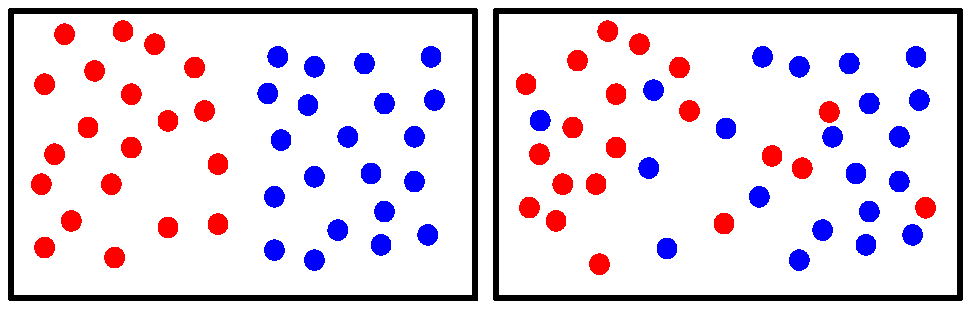
\includegraphics[width=1.0\textwidth]{fig1.pdf}

  \caption{Entropy is a property of the system. In this figure, blue and red
  particles move freely according to the time asymmetric laws of motion (if
  you don't see them moving, look closer). This figure is important to our
  discussion for two reasons. First, it is directly related to MaxEnt, which
  is an attempt to find the least biased probability distribution given a
  set of constraints by choosing the distribution with the greatest entropy
  (i.e. more like the right panel). Secondly, one of life's most dramatic
  feature is how it maintains highly organized structures \cite
  {dro01b,sel05,gol11}, essentially fighting entropy by absorbing external
  energy. The idea of life as a struggle against entropy is from Erwin Schr\"
  odinger's influential ``What is Life? '' \cite{sch44}.}

  \label{fig:entropy}
\end{figure}

\begin{figure}[h!]
  \centering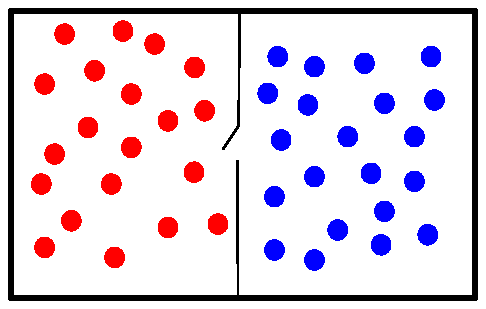
\includegraphics[width=0.6\textwidth]{fig2.pdf}

  \caption{Maxwell's demon is an apparent violation of the second law of
  thermodynamics that shed light on the relationship between entropy in
  thermodynamics and information entropy. Given a system with our gorgeous
  red/blue particles separated by a wall with a door. If the door is open,
  we have a closed system where the blue and red particles will mix,
  increasing entropy. However, what if some entity (the ``demon'')  controls
  the door. Not only could this entity prevent entropy from increasing, it
  could decrease the overall entropy by letting only red particles pass to
  the left, and the blue ones to the right. Le\'o Szil\' ard nearly resolved
  the paradox in 1929 by suggesting that the demon needed something to
  measure the behaviour of the particles. However, it took decades to
  formulate a coherent answer to Maxwell's demon, and more importantly, to
  understand the importance of information's physical nature \cite
  {lan96,kar09,gle11}. Still today, the simple paradox lies at the
  foundation of modern research on information-to-energy conversion \cite
  {toy10,wis13}.}

  \label{fig:maxwell}
\end{figure}

\subsubsection{Mathematical Definition}

Mathematically, the entropy $S$ of a system can be defined as:

\begin{equation}
   S = -k\sum_i p_i \ln p_i,
\end{equation}

with $k \equiv 1.38065e-23 J K^{-1}$ being the Boltzmann constant in statistical
physics. $p_i$ is the probability that the system is in microstate $i$ \cite{bol72}. We
get the standard equation for information entropy by setting $k = \log(2)^{-1}$ and
summing over the sample space $\Omega$:

\begin{equation}
   H(\Omega) = -\sum_{\omega \in \Omega} p_\omega \log_2 p_\omega.
\end{equation}

This measure in bits was introduced by Shannon \cite{sha48,ash65} and is
often called Shannon entropy. This concept can be applied to probability
distributions (Figure \ref{fig:entropy_dist}).

\begin{figure}[h!]
  \centering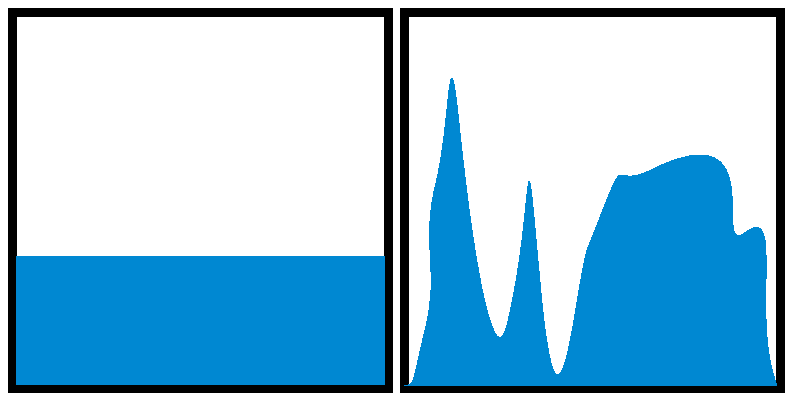
\includegraphics[width=1.0\textwidth]{entropy_dist.pdf}

  \caption{The distribution on the left has high entropy, while the distribution
  of the right is highly structured, and thus has low entropy. The intuition
  for MaxEnt is that the left panel is preferred unless we have strong evidence
  to support the complexity of the distribution on the right panel. Jaynes
  refer to this idea as ``maximum ignorance'', trying to find the distribution
  that will minimize the amount of information we cannot justify.}

  \label{fig:entropy_dist}
\end{figure}

\subsubsection{MaxEnt}

Even with such a short introduction to entropy, we can start to build an
intuition of the main idea of MaxEnt. A naive interpretation of ``maximum
entropy'' could be that we're trying to maximize ignorance. Jaynes, the
``father'' of MaxEnt, explained in his \emph{Probability Theory: The Logic
of Science} that Bayesian thinking needed a way to rigorously defined a
state of maximum ignorance, or in his humble words \cite[chpt. 12]{jay03}:

\begin{quotation}
The problem of translating prior information uniquely into a prior probability
assignment represents the as yet unfinished half of probability theory, though
the principle of maximum entropy in the preceding chapter provides one important
tool. It is unfinished because it has been rejected for many decades by those
who were unable to conceive of a probability distribution as representing
information [...]
\end{quotation}

We can compute the entropy of a probability distribution (Fig. \ref
{fig:entropy_dist}) and use it to select the best prior. According to Jaynes
\cite{jay03} (and this point is controversial \cite{che04}), MaxEnt must be
understood in the context of Bayes' theorem. Let

\begin{equation}
  p(a \mid b) \equiv \frac{p(a \cup b)}{p(b)},
\end{equation}

where $p(a)$ stands for the probability of event $a$ and $p(a \mid b)$ is
the probability of $a$ conditional on $b$. With the simple substitution $p(a
\cup b) \equiv p(b \mid a)p(a)$ we reach Bayes' theorem:

\begin{equation}
  p(a \mid b) = \frac{p(b \mid a)p(a)}{p(b)},
\end{equation}

With $\mbox{likelihood} \equiv p(b \mid a)$, we can read the theorem:

\begin{equation}
  posterior = \frac{likelihood \times prior}{evidence}.
\end{equation}

Bayes rule establishes how to compute the posterior given the prior and the
likelihood \cite{lee12}. That is, it allows us to update our belief in face
of new evidence \cite{hal05}. Jaynes argues that an equally important task
is to establish the prior \emph{uniquely}. That is, to find a systematic
method to establish the prior. This is not the only way to use MaxEnt, but
it was the primary motivation of Jaynes \cite{jay03}. To uniquely define the
least biased distribution, a mathematical tool called Lagrange multipliers
can be use. I'll quickly describe the method to help build an intuition of
how MaxEnt can be applied.

\subsection{Lagrange multipliers}\label{section-lag}

MaxEnt's core principle is to maximize the entropy of a distribution
subjected to constraints on this distribution (``maximum ignorance''). This
optimization problem requires Lagrange multipliers, a technique that will
come back in the review of the article. For a multidimensional space denoted
by $f(\mathbf{x}) \equiv f(x_{1}, x_{2}, x_{3}, ...)$, we need to find the
critical points. More formally we need to solve:

\begin{equation}
  \mbox{max}_{\mathbf{x}} f(\mathbf{x}) \mbox{ given } g(\mathbf{x}) = k.
\end{equation}

The technique has two steps. 1: Find the vector $\mathbf{x}$ and $\lambda$ such as

\begin{equation}
  \nabla f(\mathbf{x}) = \nabla \lambda g(\mathbf{x}) \mbox { and } g(\mathbf{x}) = k.
\end{equation}

For a function with $\omega$ dimensions, $\nabla f (\mathbf{x})$ is the
gradient such as:

\begin{equation}
  \nabla f (\mathbf{x}) \equiv \sum_{i = 1}^{\omega} \frac{\partial f(\mathbf{x})}{\partial x_{i}} \hat{x}_{i}.
\end{equation}

where $\hat{x}_{i}$ are orthogonal unit vectors. 2: Evaluates $f(\mathbf{x})$
for all vectors $\mathbf{x}$ found in (1). The largest value is the maximum
and the smallest value the minimum. It's also common to rewrite the problem
as an unconstrained problem \cite{gow08} by defining the Lagrangian

\begin{align}
  \mathcal{L}(\mathbf{x}, \lambda) &= f(\mathbf{x}) - \lambda g(\mathbf{x}),\\
  \nabla \mathcal{L}(\mathbf{x}, \lambda) &= k.
\end{align}

As a short example, solving $f(\mathbf{x}) = x_{1} + x_{2} + 2x_{3}$ subject to the
constraints $x_{1}^{2} + x_{2}^{2} + x_{3}^{2} = 3$ gives
$\nabla f = \langle 1, 1, 2 \rangle$ and $\nabla g = \langle 2x_{1}, 2x_{2},
2x_{3} \rangle$ \cite{ste09}. The system of equation to solve is:

\begin{align}
  1 &= 2\lambda x_{1},\label{lag-x1}\\
  2 &= 2\lambda x_{2},\label{lag-x2}\\
  2 &= 2\lambda x_{3},\label{lag-x3}\\
  x_{1}^{2} + x_{2}^{2} + x_{3}^{2} &= 3.
\end{align}

Solving the first three equations for $x$ and plugging into the fourth gives

\begin{equation}
  \frac{1}{4\lambda^2} + \frac{1}{4\lambda^2} + \frac{1}{\lambda^2} = 3
\end{equation}

or $\lambda = (2^{-1/2}, -2^{-1/2})$, and by plugging these values into
equations \ref{lag-x1}-\ref{lag-x3} we get the extrema $(\sqrt{2}/2,
\sqrt{2}/2, \sqrt{2})$ and $(-\sqrt{2}/2, -\sqrt{2}/2, -\sqrt{2})$. Dan
Klein's \emph{Lagrange Multipliers without Permanent Scarring} \cite{kle04}
offers a quick introduction to the subject with examples.

The main intuition is that MaxEnt is about optimizing entropy (or
ignorance), but it allows prior knowledge to be included in a systematic
matter as constraints on the distributions.

\subsubsection{Alternatives to MaxEnt}

MaxEnt is a technique to build a model from data. As such, it is often
compared to other algorithms from machine learning \cite{mur12} (see \cite
{has09} for an introduction to machine learning from the perspective of
traditional statistics).  In a nutshell, a machine learning method can be
seen as a function that takes evidence (data) and parameters to output a
model (itself a function that takes evidence and output predictions) \cite
{mit06,old08,mur12}. Decision trees \cite{qui86,cut07}, support vector
machines \cite{cor95}, Gaussian processes \cite{ras06}, and neural networks
\cite{ros58,sal09,hin10} are among the methods that can be used instead of
MaxEnt. All these methods have been used in ecology, in particular to the
problem of species distribution \cite{fra10}.

Comparing these methods is complicated, and how different machine learning
algorithms are related to each other is a largely unresolved issue \cite
{mit06}. They obviously share a great deal of tools from statistics and
probability theory, but as algorithms, there is no obvious way to translate,
say, a neural network to a decision tree \cite{mur12}. Although some recent
results \cite{izb13a,izb13b} suggest we might get some answers from a branch
of mathematics called category theory \cite{bar10,sim11}.

Deep learning with neural network is arguably the most popular machine
learning approach of the last few years, but it requires much tweaking and
toying to get the model right \cite{hin10}. In some ways, it is the polar
opposite of the systematic method Jaynes was looking for. Support vector
machines, on the other hand, are straightforward to use and will generally
give a solid model.

MaxEnt is a bit special in its ambition: Jaynes claims that it is the most
rational way to perform inference \cite{jay03}. Harte2008 repeats that
it is an approach based on mathematical logic, while most other methods
like neural networks are not derived from any axiomatic foundation. Reading
papers on neural networks feel like the field is performing a random walk in
the vast field of possible neural networks, but it's hard to argue against
their effectiveness.

Aside from the epidemiological question, MaxEnt shines by its ability to
easily incorporate prior information in the form of constraints. In theory,
when the constraints are defined, MaxEnt proposes a straightforward method
to generate predictions. There should be no tweaking involved. MaxEnt has
been noted for contradicting the Bayesian approach in some cases \cite
{uff96,uff95,mac03}, although this is an area of dispute \cite{jay03,che04}.

\subsection{Macroecological patterns}

Hubbell traces the roots of theoretical ecology at MacArthur and Wilson's
theory of island biogeography \cite{mac67,wil09,fle10}. The theory predicts
the number of species on an island as a function of island size and the
distance from the mainland. It implies that two main processes drive the
number of species: immigration is a function of distance (greater distance
$\Rightarrow$ less immigration), and extinction (bigger island $\Rightarrow$
less extinction). Bigger island should decrease extinction by providing more
ecological opportunities, and perhaps larger populations. Ever since,
theoretical ecology has worked to developed theories capable of predicting
several more macroecological patterns. The MaxEnt Theory of Ecology (METE)
applies MaxEnt to a number of these ecological patterns. (see Table \ref
{tab:acronyms} for a list of patterns and their acronyms).

\begin{table}
  \centering
  \begin{tabular}{ll}
    Acronym & Description \\
    \hline
    SAR & Species-area relationship \\
    EAR & Endemics-area relationship \\
    SAD & Species-abundance distribution \\
    AER & Abundance-energy relationship \\
  \end{tabular}
  \caption{A few macroecological patterns.}
  \label{tab:acronyms}
\end{table}

\subsubsection{Hubbell' Neutral Theory of Biodiversity}

There are several alternatives to METE, but Harte2012 claims Hubbell's
neutral theory of biodiversity \cite {hub01,lei07,ros11b} is closest in
spirit to the Maximum Entropy Theory of Ecology \cite[p. 208]{har12}. Like
Harte's MaxEnt theory of ecology, the unified neutral theory of biodiversity
(UNTB) can predict several macroecological patterns, with an emphasis on
species distribution abundance. Unlike METE, the neutral theory is firmly
mechanistic. It builds a theory from three mechanisms: drift, point
speciation (\emph{mutation} in population genetics), and dispersal. From
there, the UNTB borrows mathematical tools developed for sampling alleles in
population genetics \cite{mor62,ewe72}. The theory assumes that all
individuals have the same rate of birth, death, dispersal, and that they
speciate at the same rate. The theory is widely used and has been extended
in several directions \cite{all09,alo06,eti07,vol03,zho08}. It is also
controversial for assuming no differences between species \cite{cla09,pur10}
and has a mixed empirical record \cite{don06,mcg03,ric03,mcg06b}.

Two aspects of the neutral theory are interesting to keep in mind when
analyzing the METE.

First, the neutral theory is often used as a statistical model. While in
theory the UNTB is clearly based on three mechanisms, scientists often fit
the model with no regard to the actual rates of birth, death, dispersal, and
speciation. As a consequence, many fits might require rates that deviate
substantially from what is observed, or even require impossible rates (e.g.
very high rates of speciation \cite{des11}). The issue is not that the UNTB
is mechanistic or not, but the fact that it tends to be interpreted as a
mechanistic theory but used as a statistical theory. There is nothing wrong
from fitting an equation from relativistic physics to ecology as long as you
don't claim it results from the mechanisms of relativistic physics. On the
other hand the neutral theory of molecular evolution is clearly mechanistic
\cite {kim68,kin69}. It assumes that most genes are under very weak
selection defined as $s << 1/N_{e}$, with $s$ being the selection
coefficient and $N_{e}$ the effective population size). The theory is
expected to break down even if a relatively small proportion of loci\footnote
{Locus (\emph{pl. loci}): position of a sequence on a chromosome.} are
under selection \cite {kim83,gil91}.

Secondly, the METE's ambition is to generate predictions on many aspects of
macroecology. McGill et al. rightfully suggested that a good theory should
make several predictions and, of course, be judged on all these predictions
\cite{mcg07}. The neutral theory fares poorly in this respect. For example, a
recent paper by Etienne and Haegeman showed that the theory cannot generate
good predictions on speciation patterns without changing the model of
speciation, but this new model of speciation generates poor predictions on
species abundance distribution \cite{eti11}.

\subsubsection{MaxEnt in ecology}

Aside for Harte2008, MaxEnt is extensively used for species distribution
modelling \cite{fra10}. Phillips, Dudik, and Schapire presented \emph{A
maximum entropy approach to species distribution modeling} at the 21th
International Conference on Machine Learning \cite{phi04}. To apply MaxEnt
to species distribution modelling, they use the local occurrence as sample
points, the geographical region under study as the space on which the
probability distribution is defined, and environmental variables as
features. The approach has been successful and is consistently among the
best performing methods \cite{phi06,eli11}. Elith et al. 2011 \cite{eli11}
covers several applications of MaxEnt to ecological problems, including the
long-term evolution of a niche \cite{ver09} and forecasting change in
species distribution under climate change \cite{yat10}.

Shipley et al. also used MaxEnt to predict abundances from traits \cite
{shi06,shi10}. However, their approach is controversial, as it seems to
require that all the information in the prediction is already present in the
data \cite{hae08,hae09,shi09,har11,pet10}. I will come back to the
subject of using MaxEnt and traits for the proposal.

% At least 20%
\newpage
\section{Critical Review}\label{review}

In this section I briefly describe the results of the article and follow
with a critical review.

\subsection{Main results}

The METE is formulated with a few parameters: the area of the ecosystem $A_0$
, the number of individuals $N_0$ in $A_0$, the summed metabolic energy rate
of all individuals $E_0$ in $A_0$, and the number of species $S_0$ in $A_0$.
Then, the MaxEnt approach has to be applied to two distributions: $R(n,
\varepsilon)$ and $P_A^{j}(n)$. $R(n, \varepsilon)$ is the joint distribution of
species abundances $n$ and energy demand $\varepsilon$. It must satisfy the
following constraints: a normalization condition

\begin{equation}\label{rne-const1}
  \sum_{n = 1}^{N_0} = \int_0^{E_0}R(n, \varepsilon)d\varepsilon = 1,
\end{equation}

an average number of individuals per species

\begin{equation}\label{rne-const2}
  \sum_{n = 1}^{N_0} = \int_0^{E_0} nR(n, \varepsilon)d\varepsilon = \frac{N_0}{S_0},
\end{equation}

and a constraints on the average total energy requirement for a species

\begin{equation}\label{rne-const3}
  \sum_{n = 1}^{N_0} = \int_0^{E_0}n\varepsilon R(n, \varepsilon)d\varepsilon = \frac{E_0}{S_0}.
\end{equation}

Note that ``species'' is defined as a group of individuals, it can fit the
concept of biological species but can also apply to any group of individuals
\cite{coy04,har11b}. The second core distribution is $P_A^{j}(n)$. It is the
spatial abundance distribution defined as the probability of finding $n$
individuals of species $n$ within some subset $A \subseteq A_0$. This
distribution is subjected to a normalization constraint

\begin{equation}
  \sum_{n = 0}^{n_0} P^{n_0}_A(n) = 1,
\end{equation}

and to the constraint

\begin{equation}
  \sum_{n = 0}^{n_0} nP^{n_0}_A(n) = n_0\frac{A}{A_0}.
\end{equation}

From there we can defined the SAD, SED, SAR as:

\begin{equation}\label{eq-dist-1}
  SAD(n) = \int_0^{E_0} R(n, \varepsilon)d\varepsilon.
\end{equation}

\begin{equation}\label{eq-dist-2}
  AER(\varepsilon) = \frac{S_0}{N_0}\sum_{n = 1}^{N_0} nR(n, \varepsilon).
\end{equation}

\begin{equation}\label{eq-dist-3}
  SAR(A) = S_0\sum_{n = 1}^{N_0}\left[1 - P_A^{n_0}(0)\right]SAD(n_0).
\end{equation}

Using the constraints from equations \ref{rne-const1}-\ref{rne-const3}, MaxEnt
can be applied to derive $R(n, \varepsilon)$:

\begin{equation}\label{maxent-rne}
  R(n, \varepsilon) = \frac{\exp(-\lambda_1n)\exp(-\lambda_2n\varepsilon}{\sum_{n' = 1}^{N_0} \int_0^{E_0} \exp(-\lambda_1n')\exp(-\lambda_2n'\varepsilon')d\varepsilon'},
\end{equation}

With $\exp(x) \approx 2.718^x$, and $\lambda_1, \lambda_2$ being the
Lagrange multipliers explained in subsection \ref{section-lag}. There is no
closed-form solution to this equation so it must be solved numerically. Finally,
MaxEnt is applied to solve $P_A^{j}(n)$:

\begin{equation}\label{maxent-p}
  P^{n_0}_A(n) = \frac{\exp(-\lambda_pn)}{\sum_{k=0}^{n_0}\exp(-\lambda_pk)}.
\end{equation}

Equations \ref{maxent-rne}-\ref{maxent-p} lead us to the SAD, SAR, AER, EAR by solving
equations \ref{eq-dist-1}-\ref{eq-dist-3}:

\begin{equation}
  SAD(n) = \frac{\exp(-\lambda_{1}n)}{n\ln(\lambda_{1}^{-1})},
\end{equation}

\begin{equation}
  AER(n) = \frac{\lambda_{1}\lambda_{2}\exp(-(\lambda_{1} + \lambda_{2}\varepsilon))}{\left(1 - \exp(-(\lambda_{1} + \lambda_{2}\varepsilon))\right)^2},
\end{equation}

\begin{equation}
  SAR(A) = S_{0}\sum_{n_{0} = 1}\left(1 - \frac{1}{\sum \exp(-\lambda n)}\right)SAD(n_{0}),
\end{equation}

\begin{equation}
  EAR(A) = S_{0}\sum_{n_0= 1}^{N_0} \frac{\exp(-\lambda_pn_0)}{\sum_{n=1}^{n_0}\exp(-\lambda_pn)}SAD(n_0).
\end{equation}

The articles discusses some results of their predictions but do little to
compare their results with other theories. The predictions for the SAD and SAR
are good, with less opportunities to test directly the predictions for the AER
and EAR.

\subsection{Major comments}

For a ``real'' review I would suggest to accept this paper. I disagree with
some aspects of the research, but there is no major flaw in the methodology,
the article is well written, and it brings the kind of original perspective
we want in a ``Concept \& Synthesis''.

``Statistical modeling: the two cultures'' by Leo Breiman was one of the
most debated article in statistics \cite{bre01,nor11}. In it, Breiman argues
that statistics could be divided in two cultures: the data modelling culture
and the algorithmic modelling Culture. The data modelling culture is the
oldest and starts with assuming a stochastic data model. The algorithmic
culture assumes the true model is complex and focuses on algorithms capable
of building a good predictive model. This perspective is driving much of the
``Big Data'' movement \cite {hal09} and Harte2008 is a great contribution to
this perspective of data science. While MaxEnt is straightforward to apply
once we have established the variables and the constraints, Harte2008 has
the merit of (1) finding a good set of variables, (2) establishing the
constraints, and (3) of bringing a tool from a different field (the
application of MaxEnt in Harte2008 is quite different from what is done in
species distribution modelling).

\subsubsection{The place of mechanisms}

Ultimately, whether a scientist embrace or reject the MaxEnt approach is
likely to depend on MaxEnt's predictive power, and her/his view of
mechanistic models. Is the approach capable generating good predictions?
Impressive results for MaxEnt in species distribution modelling shows the
method has a place in ecology \cite {fra10,eti11}. Even if these results are
based on a different application of MaxEnt, they will likely help promote
the idea. With the benefit of hindsight, we can also say the theory fare
well: it survived tough tests \cite{xia13} and has been extended \cite
{whi12,mcg13}. However, testing is barely covered in the article.

The second question is the place of mechanisms: MaxEnt does not start with
any assumptions about the mechanisms involved. Harte2008 defended well this
aspect of their theory. There have been calls to adopt a more pragmatic view
of mechanisms \cite{mcg10}. If a mechanistic approach gives good
predictions, let's adopt it, but if a machine learning method gives better
results, there is no reason to reject it on the ground that it does not
involve mechanisms. I was already sold to this argument, and I think Harte
made a good case against a systematic bias in favour of mechanistic model in
his book \cite{har11}. The authors also pointed out that MaxEnt can allow
mechanisms to be involved if they can be described as a constraints. Still,
the lack of mechanisms will likely remain quite controversial (see \cite
{tur03,cla09,wen12}). Ecology is still divided on the methods and approach
to use for building theories. For example, in ``How Planets Move and
Populations Grow'', Ginzburg and Colyvan argue that populations should be
studied with second-order deterministic different equations \cite
{gin86,gin04}. Ginzburg's philosophy of modelling is further explored in a
2004 paper published in \emph{Trends in Ecology \& Evolution} \cite {gin04b}.

\subsubsection{Axioms, mathematical rigour, and ad hoc-ness}

In her book on species distribution models, Franklin places MaxEnt in the
chapter on machine learning methods \cite{fra10}, along with decision trees,
artificial neural networks, and genetic algorithms. From this perspective,
MaxEnt is simply one among many machine learning methods. This is a common
view of MaxEnt. For example, in natural language processing, MaxEnt is
favoured for many tasks including part-of-speech tagging, the problem of
classifying a word given its context \cite{man99}.

The authors could easily have defended MaxEnt as a method, ignoring the
epidemiological debate... but they didn't. In fact, they chose to put the
epidemiological debate front and center of their theory. In the introduction
to the article, the authors \emph{emphasize that making predictions using
MaxEnt is an application of mathematical logic. It is a rigorously proven
mathematical procedure for inferring the most likely probability
distribution, if our knowledge about that distribution can be incorporated
as a set of constraints on the distribution.} And in the discussion, they
\emph{re-emphasize that MaxEnt is a mathematically proven method for
inferring the most likely probability distribution if our knowledge about
that distribution can be described as a set of constraints on the
distribution.} Furthermore, the book devotes almost an entire chapter to
this issue, and the recent opinion piece in \emph{Trends in Ecology \&
Evolution} also makes this point. Jaynes' ``Probability: the logic
of science'' offers a similar perspective on MaxEnt \cite{jay03}.

``Mathematically proven'' does not mean much. A mathematical proof requires
an axiomatic system. An axiom is something we accept as true and cannot
prove. Zermelo-Fraenkel set theory provides the most important axiomatic
system in mathematics \cite{and94}, but one axiom (i.e. the axiom of choice)
is controversial \cite {pen05} and new foundations for mathematics are being
established \cite {bar05,awo11,ufp13}. MaxEnt is only proven under a
recently established set of axioms \cite {har11}. To emphasize: the
axiomatic approach is very interesting since it forces us to clearly
establish our foundation for reasoning and derive results only from these
foundations. However, history has showed that building a good axiomatic
system is difficult, and probability theory is no exception \cite
{cox46,mac03,gha05}. Any theorem can be proven within some axiomatic system
\cite{and94}. Furthermore, G\"odel \cite{god62} showed how this approach was
limited: an axiomatic system cannot demonstrate its own consistency. Thus,
the fact that MaxEnt is proven under a recently established axiomatic system
(which was essentially designed to prove MaxEnt), is rather unimpressive.
Not only the article emphasizes this aspect repeatedly, they claim that
MaxEnt can only fail by assuming incoherent constraints or ignoring
important ones. MaxEnt can also fail because its axioms are inappropriate
for a given problem. Inference cannot be made without assumptions, and we
have no reason to think that a single inference system is optimal in all
cases \cite{mac03}. To his credit, Harte does mention the possibility that
failure is caused by the axioms \cite [p. 130] {har11}, but it is not
mentioned in the recent opinion piece \cite {har14} (which, again, says that
MaxEnt is a mathematically proven procedure).

As an example of a reasonable alternative to MaxEnt: entropy might not be
the best tool to find the least biased distributions. Minimum description
length and Kolmogorov complexity are possible alternatives with their own
success stories \cite {kol65,gru03,li_08,mit09,yua13}. Perhaps more
importantly, MaxEnt does not need to be mathematically proven. Neural
networks are arguably the most successful methods in machine learning at the
moment. Yet, getting a neural networks to work well is notoriously difficult
and requires many arbitrary choices \cite{hin06}.

\subsection{Minor comments}

Harte2008 describe two possible state variables: individuals and
``species''. Their definition of ``species'' is puzzling at best, since it
can be applied not only to species but to any group of individuals. Using
the term ``species'' implies the theory is less general than it really is. A
species is generally defined as an interbreeding group of individuals (plus
or minus a few controversies \cite{coy04}). Harte2008's species is a strict
superset of the standard species concept: everything recognized as a
species with the standard definition fits Harte2008's ``species'', but all
other grouping of individuals fit too. The authors probably chose the term
because it is the most common set of group available, but using a more general
term would be more accurate.

% At least 30%
\newpage
\section{Proposal}\label{proposal}

In this section, I will propose a research plan to extend the framework
established by Harte et al. 2008 \cite{har08}. I present an idea for a
theoretical project to derive constraints from evolutionary theory and apply
them to the METE. I finish this section with a simple alternative project
idea.

\subsection{Introduction}

Harte and Newman \cite{har14} suggests rapid evolutionary changes can
explain some of the important deviations from MaxEnt \cite{har14}. It begs
the question: can we find a more general framework that would unify
community ecology and evolutionary biology? In this section, I propose a
project to unify the MaxEnt theory of ecology with evolutionary theory using
the most useless and inapplicable equation found in theoretical population
genetics.

\subsection{Background}

Population genetics has strong foundations in Mendelian genetics \cite
{cha11b}. The most basic processes of evolution are well-known and
understood: mutation, recombination, selection, drift \cite
{cro70,lyn07,gil04b,gil04b}, and perhaps random genetic draft as well \cite
{gil01}. Unfortunately, the last few decades showed that a powerful model
for theoretical population genetics needed to incorporate the fact that
selection varies in both time and space \cite
{gil01,beg07,bel08,bel09,bel10}. This task is difficult because of the sheer
number of parameters involved to describe this type of stochastic selection
\cite {hah08,wak05} (see \cite{gil04} for an epic attempt). If we are unable
to describe evolution at this level, integrating it in ecology seems even
more difficult.

Yet there are good motivations to integrate ecology and evolution. Not only
Harte \& Newman describe evolutionary dynamics as a potential opportunity to
improve METE's accuracy, but evolution provides a foundation for the
maintenance of individual differences (see ``An evolutionary ecology of
individual differences''\cite{dal12}). If the great mystery of life is how
it thrives ``so far from the equilibrium'' and maintains highly ordered
structures, then ecology cannot answer it without integrating evolution \cite
{gol11}. Some processes thought to be of great importance to the maintenance
of diversity, such as environmental plasticity, need to be framed within
evolutionary theory \cite {wes89,wes03,rof97}.

Unification is easier said than done. Evolution is described as a set of
processes (or mechanisms, or forces). To include them in METE, we need to
derive constraints from these processes. Since evolutionary theory is based
on population genetics, and since population genetics has no well-established theory to
offer us, how can we introduce these processes?

For this proposal, I suggest a theoretical project aimed at unifying METE
and evolutionary theory by defining constraints for MaxEnt using the
probabilistic Price equation (described in section \ref{pro:price}). One of
MaxEnt's greatest strength is to offer a simple method to get a good model
when the variables and constraints are described. Constraints cannot always
be described easily (see \cite{uff95,uff96} for detailed discussions of
constraints in MaxEnt). My proposal focuses on the theoretical development
of a framework that would allow the integration of various aspects of
evolution into the METE, with a particular emphasis on how mathematical
tools from evolutionary theory could be used as constraints on distribution
in the MaxEnt sense. I focus on a well-known and theoretically mature
equation: the Prince theorem. The Price theorem is too flexible to be used
directly, but I suggest that the probabilistic version is the most promising
avenue to add constraints based on evolution to the METE.

\subsection{Objectives}

To use the MaxEnt approach we need (1) a set of variables ($ASNE$ in the
original METE) and (2) a set of constraints for those variables. The Price
equation, even in its stochastic form, is too flexible and involve many
parameters. It is the price to pay (no pun intended) for a flexible
approach, but in this case it could help develop applications to various
problems. The approach I suggest is meta-theoretical, instead of trying to
build a single theory with a set of variables, I think integration with
evolution should aim to develop bridges between the probabilistic Price
theorem and METE. As far as I know, nothing like this has been attempted,
yet the approach offers clear advantages: the probabilistic Price equation
is not used often because it can only describe constraints (the relationship
between various distribution), but this is precisely what we are looking for.

The primary objective is thus to develop the mathematical tools to
translate the various components of the probabilistic Price theorem into
constraints for the METE. The project could be divided in two objectives:

\begin{itemize}
  \item Reframe the foundations of the probabilistic Price theorem so the
  theorem could be application to ecology.
  \item Define how constraints on the distribution of fitness, migrants, and
  the other components of the Price theorem are to be applied to the $ASNE$
  variables (or to an extended set of variables).
\end{itemize}

\subsection{Foundations}\label{pro:price}

In this section I will explain the probabilistic Price theorem. This is the
foundation to the theoretical work suggested. Let $\phi$ be a phenotype or a
vector of phenotypes. Here, a phenotype is broadly described as a measurable
trait in a species: body size, aggressivity, hair color. In this definition,
a genotype is also a phenotype since it can be measured. Genotypes and
phenotypes are often considered distinct \cite{gri08}, but this definition
of phenotype is more general and quite common for the Price theorem \cite
{ric04}. We require that $\phi$ can be described with real numbers, i.e.
$\phi \in \mathbb{R}$.

To derive the Price theorem, we need a few axioms. I do not pretend that the
Price theorem is ``mathematically proven'' or more rigorous because it is
based on axioms, but it does establish clearly what we need to find the
theorem. Many models in population genetics start with many explicit and
implicit assumptions, such as fixed population size and constant selection,
we will avoid these strong assumptions to ensure the MaxEnt's emphasis on
``maximizing ignorance'' \cite{jay03} is not disrupted. I use a slightly
modified version of Rice's axioms \cite{ric09}:

\begin{itemize}

  \item A0. Our object of study is a set of individuals.

  \item A1. Each individual can be described as a set of phenotypes.

  \item A2. Individuals leave descendants such that we could, in principle,
  identify which descendants came from which ancestors. As in the Fisher \cite{fis58} and
  Price equations \cite{fra95}, an individual can count itself at a future time as a
  descendant.

  \item A3. Each individual within a population has a probability
  distribution of possible numbers of descendants that it could leave after
  a specified time interval. This fitness distribution is causally
  influenced by both the individual's phenotype and its environment. This
  includes both biotic and abiotic environments.

  \item A4. Each individual has a distribution of possible descendant
  phenotypes. This distribution is causally influenced by the individual's
  phenotype, its environment, the transmission process (genetic and
  cultural), and the development of the descendants themselves.

\end{itemize}

I will first explain the deterministic Price theorem \cite
{pri70,pri72,pri72b,fra12} and follow with a discussion of the probabilistic
Price theorem derived by Rice \cite{ric04,ric08,ric09}. See table \ref
{tab:symbols} for a list of symbols used. An explanation of the
probabilistic Price equation is beyond the scope of this text, see \cite
{ric09} for a complete derivation. However, we can get an intuition of the
probabilistic equation from the deterministic Price theorem.

\begin{table}
  \centering
  \begin{tabular}{cl}
    Symbol              & Description \\
    \hline
    $N$                 & Population size \\
    $\phi_i$            & Phenotype of the $i$th individual. \\
    $\bar{\phi}$        & Mean phenotype of a population. \\
    $\delta_{i,j}$      & Difference between the phenotype of the ancestor $i$ and its $j$th descendant.\\
    $\bar{\delta_{i}}$  & Mean difference between the phenotype of $i$ and its descendants.\\
    $W_{i}$             & Number of descendants for $i$.\\
    $\bar{W}$           & Mean number of descendants.
  \end{tabular}
  \caption{Symbols for the deterministic and probabilistic Price theorem.}
  \label{tab:symbols}
\end{table}

The first formulation of the Price equation is intuitive, we first defined
the phenotype at time $t + \Delta t$ as $\phi'$ and simply get the new
average phenotype by adding the phenotype of the next generation:

\begin{equation}
  \bar{\phi'} = \frac{\sum_{i=1}^{N}\sum_{j=1}^{W_{i}}\left(\phi_{i} + \delta_{i,j}\right)}{\sum_{i=1}^{N} W_{i}}.
\end{equation}

We can rewrite using the definition of the mean as

\begin{equation}
  \bar{\phi'} = \frac{1}{\bar{W}}\left(E(W\phi) + E(W\bar{\delta})\right),
\end{equation}

and finally, using the fact that $\mbox{cov}(x, y) = E(xy) - \bar{x} \times
\bar{y}$ and defining $\Delta \bar{\phi} = \bar{\phi'} - \bar{\phi}$, we
get the Price theorem for the variation of a phenotype between the ancestors
and their descendants:

\begin{equation}\label{primcetheorem}
  \Delta \bar{\phi} = \frac{1}{\bar{W}}\left(\mbox{cov}(W, \phi) + E(W\bar{\delta})\right).
\end{equation}

Here, covariance ($\mbox{cov}$) is an exact measure, it is not an estimate.
See figure \ref{fig:price} for an illustration of the theorem. Of course,
the issue is that we need to know the phenotype of all descendants, making
the theorem somewhat useless. Unsurprisingly, there are many debates about
the importance of this theorem \cite{ewe04,oka08,fra12}.

Now that we have the deterministic Price theorem, how can it be useful to
us? In essence, equation \ref{primcetheorem} describes how the phenotype
evolves from the ancestors to their descendants. Much of the interesting
dynamics lies in $\mbox{cov}(W, \phi)$, and a great deal of work has been
done on studying selection, drift, and the other mechanisms within this
framework \cite{ric04}. This is a key point: we are not trying to re-derive
a theory of evolution. Also, the central equation of quantitative genetics,
the Breeder' equation, can be reached by assuming that the relationship
between the ancestors and their descendants is a linear regression with
noise \cite{lyn98}.

The probabilistic version \cite{ric08} redefines everything in terms
of probability distributions and discovers many relationships that can
be described as constraints on the distribution of traits. A few example
of the relationships found \cite{ric09}:

\begin{itemize}

  \item C0. In a closed population (no migration), change in mean phenotype is
  inversely proportional to mean population fitness.

  \item C1. In an open population (with immigrants), change in mean phenotype is
  inversely proportional to the per capita growth rate.

  \item C2. In the absence of correlation between propensity to emigrate and
  phenotype, increasing emigration reduces the intensity of selection.

  \item C3. If the offspring of poorly adapted ancestors have a higher
  propensity to emigate, the intensity of directional selection increases.

  \item C4. Covariance between emigration and phenotype essentially behaves like
  selection.

  \item C5. The distribution of migration rates has a strong effect on the
  potential for local adaptation.

\end{itemize}

These are just a few of many relationships found in the probabilistic Price
theorem. Some of these relationships are well known \cite{hed04,cha11b}, but
the probabilistic Price theorem describes them precisely as constraints on
probability distributions. From there, we only need two breakthroughs to
introduce them into the METE. First, since the probabilistic Price theorem
is almost infinitely flexible, we need to identify data-sets where some of
these constraints are known. Then, we need to relate these constraints to
the variables of the METE. Adding a state variable for traits in the METE
will likely be necessary to get the most our of the probabilistic Price
theorem.

\begin{figure}[h!]
  \centering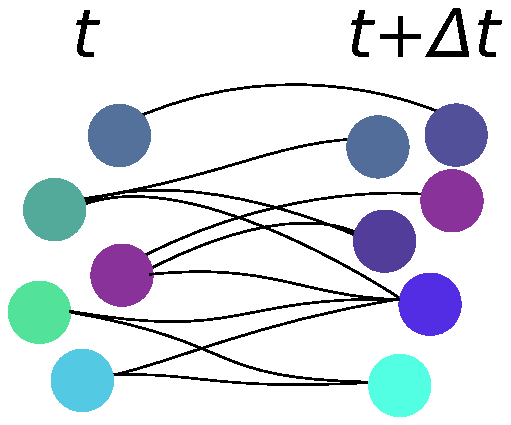
\includegraphics[width=1.0\textwidth]{price.pdf}

  \caption{The scope of the Price equation \cite{fra12}. On the left,
  individuals with different traits at time $t$. The Price equation follows
  the evolution of the individual for some arbitrary $\Delta t$. The
  equation does not assume overlapping or non-overlapping population
  dynamics: it assumes only that all descendant can be mapped to one or more
  ancestors. In an individual survives the time interval, it can be its own
  ancestor. We also see an individual with 4 ancestors (grandparents). This
  flexibility fits well in a probabilistic framework \cite{ric08} where
  we are interested in the probability distribution of descendants. Each individual
  can be defined with one or more real-valued traits.}

  \label{fig:price}
\end{figure}

The Price theorem has been used in ecology for a different purpose, namely
to understand on species loss affects ecosystem function \cite{fox06,fox08}.
Nothing in the Price theorem prevent it from dealing with individuals from
different species or applied to an entire community. The Price theorem is
also related to Fisher's fundamental theorem of natural selection \cite
{fis30,fis58}, recently revised \cite{les97}. See \cite{oka08} and \cite
{ewe04} for reviews of Fisher's theorem.

\subsection{Expected results}

The main issue with the probabilistic Price theorem is that it can \emph
{only} describe constraints and require too much information about the
distribution of traits, immigration, and emigration. However, this framework
fits perfectly with MaxEnt because it makes no strong assumptions about how
populations behave. Many of the problems with theoretical population
genetics are related to the difficulty of finding the right simplifying
assumptions. The neutral theory assumes that most variation is causes by
neutral processes \cite{kim83,oht96}, while models with selection need to
make strong (and hard to justify) assumptions about selection \cite{gil01}.
MaxEnt works well because it starts from a state of ``ignorance''. Having a
framework with unreliable assumptions would introduce bias, so any attempt
to integrate evolution through theories such as the neural theory of
molecular evolution are unlikely to work.

Theoretical work is always risky and I can see two major roadblocks, two
ways this project could fail. First, there is the possibility that the
constraints in the probabilistic Price equation cannot be translated into
constraints for an ecological theory, perhaps because traits would be
difficult to introduce as state variable in a way that would fit both the
METE and the Price theorem. I doubt this would be a real difficulty. Ecology
and evolution can meet with the $N$ part of METE's $ASNE$ in two ways: the
Price theorem can be applied to the community as a whole, or we can derive a
community as a set of populations. While Shipley's approach to traits seems
flawed in some respects, it shows some potentially useful ways to think about
traits within MaxEnt \cite{shi10}.

The second roadblock for integrating the Price theorem is testing. In
theory, there is no reason why this approach could not be tested. In fact,
the approach should enable a great number of variants of METE and expand the
number of possible predictions. The problem is cultural. Theoretical work in
evolution tends to focus on predicting patterns of molecular evolution, even
when the subject is adaptation \cite{orr02,wil12}. Similarly, macroecology
tends to ignore evolution, focusing on a pattern with little regard to its
formation or long-term dynamics \cite{mcp07,ric08b}. As a consequence, even
though ecology and evolution are often difficult to differentiate (e.g. is
selection an ecological process?), both fields have been focusing on
specific predictions that almost completely exclude each other. This is not
to say that testing an eco-evolutionary theory is impossible, but it has not
been a major focus of either communities.

At the very least, I think \emph{trying} to make the unusable Price theorem
usable through MaxEnt would be productive. The approach seems original, and
the almost complete lack of simplifying assumptions makes the Price theorem
flexible. Since it does nothing but define constraints on distributions, it
might be a perfect fit for MaxEnt. There is a reasonable chance that even a
failure would open a path toward an evolutionary METE \cite{lyn98}.

\subsection{An alternative: Constraints and transfer}

As scientists accumulate more and more data, the problem of building bridges
between different pieces of data becomes more important \cite
{tan06,hal09,rus09}. MaxEnt allows us to introduce prior knowledge with
constraints. Thus, it seems MaxEnt would be a key tool for transfer and the
``Big Data'' age. Yet, the most ambitious form of knowledge transfer is
about dealing with arbitrately different pieces of information \cite
{mil07,dav09,dom09}. It's not obvious at all how MaxEnt could deal with
arbitrarily different data. To scale to large heterogeneous data-sets, a
method needs two things. First, it needs to find relevant data. Second, it
needs to establish how the data can be use with other pieces of data. The
first step it outside the scope of MaxEnt but could be done with a different
tool, and the second implies a system to define constraints automatically.
To see why this is difficult, consider the Kullback–Leibler divergence \cite
{kul51}:

\begin{equation}
 KL(p\|q) = \int_{-\infty}^\infty \ln\left(\frac{p(x)}{q(x)}\right) p(x)dx.
\end{equation}

$KL$ measures relative entropy, or the difference between two probability
distributions (it's not a metric since $KL(p\|q)$ is not always the same as
$KL(q\|p)$ \cite {tho08,tao11}). Note that $KL(p\|q)$ is undefined for
arbitrarily different distributions. However, from the perspective of
knowledge transfer, you need to estimate the distance between two pieces of
information, even if they appear unrelated. The primary ambition of MaxEnt
is to uniquely describe the best prior for a given problem, which seems like
a tricky thing to do for knowledge transfer.

I would be interested to know if there is a way to use the MaxEnt approach
for this problem. If transfer could be achieved with MaxEnt, testing should
be relatively simple. Some important deviations of MaxEnt has been observed
in some cases, and Harte suggest that additional constraints could be used
\cite{har14}. A general solution to these extreme cases would need a system
to automatically add constraints, that is: to transfer knowledge.

\newpage
\bibliography{refs}
\bibliographystyle{plain}
\addcontentsline{toc}{section}{References}

\end{document}
